\documentclass[]{article}

\usepackage[margin=1.5in]{geometry}
\usepackage[utf8]{inputenc} % this is needed for umlauts
\usepackage[ngerman]{babel} % this is needed for umlauts
\usepackage[T1]{fontenc}    % this is needed for correct output of umlauts in pdf
\usepackage{lmodern}
\usepackage{amsmath}
\usepackage{amssymb}
\usepackage{bm}
\usepackage{amsthm}
\usepackage{hyperref}
\usepackage{mdframed}
\usepackage{xcolor}
\usepackage{graphicx}
\usepackage{caption, subcaption}
\usepackage{float}

\newcommand{\Pb}{\mathbb{P}}
\newcommand{\E}{\mathbb{E}}
\newcommand{\R}{\mathbb{R}}
\newcommand{\N}{\mathbb{N}}
\newcommand{\X}{\mathbf{X}}
\newcommand{\Y}{\mathbf{Y}}
\newcommand{\T}{\mathbf{\Theta}}
\newcommand{\muu}{\bm{\mu}}
\newcommand{\Ssigma}{\mathbf{\Sigma}}
\newcommand{\vv}{\mathbf{v}}
\newcommand{\uu}{\mathbf{u}}
\newcommand{\C}{\mathbf{C}}
\newcommand{\rk}{\mathrm{rk}}
\newcommand{\A}{\mathbf{A}}
\newcommand{\B}{\mathbf{B}}
\newcommand{\Ggamma}{\mathbf{\Gamma}}
\newcommand{\tr}{\mathrm{tr}}
\newcommand{\xx}{\mathbf{x}}
\newcommand{\yy}{\mathbf{y}}
\newcommand{\XX}{\mathcal{X}}
\newcommand{\YY}{\mathcal{Y}}

\newmdtheoremenv[backgroundcolor=black!5, innertopmargin=-2pt]{definition}{Definition}[section]
\newmdtheoremenv[backgroundcolor=black!5, innertopmargin=-2pt]{theorem}[definition]{Satz}
\newmdtheoremenv[backgroundcolor=black!5, innertopmargin=-2pt]{lemma}[definition]{Lemma}
\newtheorem*{remark}{Bemerkung}
\newtheorem*{remarks}{Bemerkungen}
\DeclareMathOperator*{\argmin}{argmin}

%opening
\title{Reduced-Rank-Regression}
\author{Daniel Herbst}
\date{10. Mai 2021}

\begin{document}

\maketitle

\begin{abstract}
Nachdem in der vorigen Präsentation das multivariate Regressionsmodell mit festen Inputvariablen vorgestellt wurde, möchten wir uns nun dem Fall zufälliger Inputvariablen zuwenden. Zudem werden wir eine Verallgemeinerung des multivariaten Regressionsmodells, das
\textit{Reduced-Rank-Regressionsmodell (RRR)}, betrachten, bei dem wir zusätzlich den Rang der Regressionskoeffizientenmatrix einschänken. Dieses Verfahren verallgemeinert unter anderem auch einige Techniken der multivariaten Statistik, etwa die Hauptkomponentenanalyse zur Dimensionsreduktion. Im Wesentlichen folgt der Vortrag 
\cite[Kapitel 6.3]{Iz08}.
\end{abstract}

\section{Einleitung}
\label{Einleitung}
Unsere Ausgangssituation ist die Folgende:
$$\X := (X_1, \dots, X_r)^\top \quad \text{und} \quad \Y := (Y_1, \dots, Y_s)^\top$$
seien Zufallsvektoren mit gemeinsamer Verteilung $\Pb^{(\X, \Y)}$, wobei $r, s \in \N$ mit $s \leq r$,
und ferner definieren wir folgende Schreibweisen für die entsprechenden Erwartungwerte und Kovarianzmatrizen (deren Existenz wir voraussetzen):
$$ \muu_\X := \E\X, \quad \muu_\Y := \E\Y \quad \text{und} \quad \begin{pmatrix}
	\Ssigma_{\X\X} & \Ssigma_{\X\Y} \\
	\Ssigma_{\Y\X} & \Ssigma_{\Y\Y}
\end{pmatrix} := \Sigma \biggl(\begin{pmatrix}
\X \\
\Y
\end{pmatrix}\biggr).$$
Abgesehen von $\Pb^\X \ll \lambda^r$ und $\Pb^\Y \ll \lambda^s$, d.h. der Stetigkeit der Zufallsvektoren $\X$ und $\Y$, möchten wir zunächst keine
weiteren Annahmen über die Verteilungen von $\X$ und $\Y$ treffen.

\section{Klassisches multivariates Regressionsmodell mit zufälliger Inputvariable}

Das klassische multivariate Regressionsmodell mit zufälliger Inputvariable ist von folgender Form: Für $\X$ und $\Y$ gelte
\[ \Y = \muu + \T \X + \mathcal{E} \text{,} \label{eq:2.1} \tag{2.1}\]
wobei $\muu \in \R^s$ und $\T \in \R^{s \times r}$ unbekannte Parameter seien sowie $\mathcal{E}$ ein (nicht beobachtbarer) $s$-dimensionaler zufälliger Fehler ist mit Erwartungswert $\E \mathcal{E} = 0$ und Kovarianzmatrix $\Ssigma_{\mathcal{E} \mathcal{E}}$. Zudem werden $\X$ und
$\mathcal{E}$ als unkorreliert vorausgesetzt.
\\

Wir möchten nun optimale $\muu$ und $\T$ finden in dem Sinne, dass die symmetrische, positiv semidefinite Matrix
$$W(\muu, \T) := \E[(\Y - \muu - \T \X)(\Y - \muu - \T \X)^\top] \in \R^{s \times s}$$ in gewisser Weise minimiert wird. Hierfür verwenden wir folgende Halbordnung, die man auf dem Raum der symmetrischen $s \times s$-Matrizen definieren kann:

\begin{definition}[Löwner-Halbordnung]
	Sei $V:= \{\A \in \R^{s \times s} \;|\; \A^\top = \A \}$ der Raum der symmetrischen $s \times s$-Matrizen. Setze für $\A, \B \in V$:
	$$\A \leq_L \B \; :\Leftrightarrow \; \B - \A \text{ positiv semidefinit.}$$
	Es lässt sich leicht nachprüfen, dass diese Relation eine Halbordnung auf $V$, die sogenannte Löwner-Halbordnung, definiert.
\end{definition}
Mit dieser Halbordnung können wir nun den folgenden Satz formulieren:
\begin{theorem}
	\label{thm:mr}
	Seien $\X$ und $\Y$ wie in der \nameref{Einleitung}, so ist
	$$ \argmin_{(\muu, \T)} W(\muu, \T) = (\muu_\Y - \T \muu_\X, \Ssigma_{\Y\X} \Ssigma_{\X\X}^{-1}) =: (\muu_{\min}, \T_{\min}) \text{,} $$
	wobei bezüglich $\leq_L$ minimiert wird. Zudem ist
	$$W(\muu_{\min}, \T_{\min}) = \Ssigma_{\Y\Y} - \Ssigma_{\Y\X} \Ssigma_{\X\X}^{-1} \Ssigma_{\X\Y} \text{.}$$
	Ferner gilt für $\mathcal{E} := \Y - \muu_{\min} - \T_{\min} \X$, dass 
	$$\E \mathcal{E} = \mathbf{0} \quad \text{und} \quad \E[\mathcal{E}(\X - \muu_\X)^\top] = \mathbf{0} \text{,}$$
	d.h. $\X$ und $\mathcal{E}$ sind unkorreliert.
\end{theorem} 

\begin{remarks}
	\hfill
	\normalfont
	\begin{itemize}
		\item Dass $(\muu_{\min}, \T_{\min})$ $W(\muu, \T)$ minimiert, soll hier natürlich \textbf{nicht} wie etwa in der Mengenlehre bedeuten, dass $W(\muu_{\min}, \T_{\min})$ ein minimales Element der Menge $\mathcal{S} := \{W(\muu, \T) \;|\; \muu \in \R^s, \T \in \R^{s \times r}\}$ ist, sondern die stärkere Bedingung, dass 
		$$W(\muu_{\min}, \T_{\min}) \leq_L W(\muu, \T) \quad \forall \muu \in \R^s, \T \in \R^{s \times r} \text{.}$$
		Insbesondere kann es nur eine Minimalstelle geben.
		\item Die Stetigkeit von $\X$ und $\Y$ sichert, dass $\Ssigma_{\X\X}$ (und $\Ssigma_{\Y\Y}$) invertierbar sind: Denn wäre $\Ssigma_{\X\X}$ singulär, so gäbe es ein $\vv \in \R^s \setminus \{0\}$ mit $$\vv^\top \Ssigma_{\X\X} \vv = \E [\| \vv^\top (\X - \muu_{\X}) \|_2] = 0 \text{,}$$
		d.h. $$\Pb(\vv^\top (\X - \muu_{\X}) = 0) = 1$$
		und die Verteilung von $\X$ ist auf einer Hyperebene konzentriert (analog für $\Y$). 
		\item Mit dem Satz von Courant-Fischer \cite[Seite 52 f.]{Iz08} lässt sich zeigen, dass, falls $\lambda_j(\A)$ der $j$-größte Eigenwert von $\A \in \R^{s\times s}$ ist, dann
		$$\A \leq_L \B \; \implies \; \lambda_j(\A) \leq \lambda_j(\B),  \quad j=1, \dots,s \text{.}$$
		Damit minimiert $(\muu_{\min}, \T_{\min})$ auch 
		\[\tr(W(\muu, \T)) = \E[(\Y - \muu - \T \X)^{\top} (\Y - \muu - \T \X)] \text{,} \label{eq:2.2} \tag{2.2}\]
		was häufig als Minimierungsbedingung bei der multivariaten Regression genutzt wird. Die hier vorgestellte Variante ist also allgemeiner.
	\end{itemize}
\end{remarks}

\begin{proof}
	Mit $\X_c := \X - \muu_\X$, $\Y_c := \Y - \muu_\Y$ gilt für alle $\T \in \R^{s \times r}$, $\muu \in \R^s$:
	\begin{align*}
		W(\muu, \T) ={}& \E[(\Y - \muu - \T \X)(\Y - \muu - \T \X)^\top] \\
		={}& \E[(\Y_c - \T \X_c + (\muu_\Y - \T \muu_\X - \muu))(\Y_c - \T \X_c + (\muu_\Y - \T \muu_\X - \muu))^\top] \\
		={}& \E[\Y_c \Y_c^\top - \Y_c \X_c^\top \T^\top + \Y_c (\muu_\Y - \T \muu_\X - \muu)^\top \\
		& \quad - \T \X_c \Y_c^\top + \T \X_c \X_c^\top \T^\top - \T \X_c (\muu_\Y - \T \muu_\X - \muu)^\top \\
		& \quad + (\muu_\Y - \T \muu_\X - \muu) \Y_c^\top - (\muu_\Y - \T \muu_\X - \muu) \X_c^\top \T^\top \\
		& \quad + (\muu_\Y - \T \muu_\X - \muu)(\muu_\Y - \T \muu_\X - \muu)^\top] \\
		={}& \Ssigma_{\Y\Y} - \Ssigma_{\Y\X} \T^\top - \T \Ssigma_{\X\Y} + \T \Ssigma_{\X\X} \T^\top \\
		& \quad + (\muu_\Y - \T \muu_\X - \muu)(\muu_\Y - \T \muu_\X - \muu)^\top \\
		={}& \Ssigma_{\Y\Y} - \Ssigma_{\Y\X} \Ssigma_{\X\X}^{-1} \Ssigma_{\X\Y} \\
		& \quad + \underbrace{(\Ssigma_{\Y\X} \Ssigma_{\X\X}^{-1/2} - \T \Ssigma_{\X\X}^{1/2})(\Ssigma_{\Y\X} \Ssigma_{\X\X}^{-1/2} - \T \Ssigma_{\X\X}^{1/2})^\top}_{=: A(\T) \quad \text{ positiv semidefinit}} \\
		& \quad + \underbrace{(\muu_\Y - \T \muu_\X - \muu)(\muu_\Y - \T \muu_\X - \muu)^\top}_{=:B(\muu, \T) \quad \text{positiv semidefinit}} \\
		\geq{}& \Ssigma_{\Y\Y} - \Ssigma_{\Y\X} \Ssigma_{\X\X}^{-1} \Ssigma_{\X\Y} \text{,}
	\end{align*}
	mit Gleichheit falls $A(\T) = B(\muu, \T) = 0$, was der Fall ist, wenn
	$$ \muu = \muu_\Y - \T \muu_\X =: \muu_{\min} \quad \text{und} \quad \T = \Ssigma_{\Y\X} \Ssigma_{\X\X}^{-1} =: \T_{\min} \text{.}$$
	Man erhält nun
	\begin{align*}
		\mathcal{E} ={}& \Y - \muu_{\min} - \T_{\min} \X \\
		={}& \Y - (\muu_\Y - (\Ssigma_{\Y\X} \Ssigma_{\X\X}^{-1}) \muu_\X) - (\Ssigma_{\Y\X} \Ssigma_{\X\X}^{-1}) \X \\
		={}& \Y_c - \Ssigma_{\Y\X} \Ssigma_{\X\X}^{-1} \X_c
	\end{align*}
	und es gilt offensichtlich $\E \mathcal{E} = \mathbf{0}$ sowie
	$$\E[\mathcal{E} \X_c^\top] = \E[(\Y_c - \Ssigma_{\Y\X} \Ssigma_{\X\X}^{-1} \X_c) \X_c^\top] = \Ssigma_{\Y\X} - \Ssigma_{\Y\X}\Ssigma_{\X\X}^{-1} \Ssigma_{\X\X} = \mathbf{0} \text{,}$$
	d.h. $\X$ und $\mathcal{E}$ sind unkorreliert.
\end{proof}

\section{Reduced-Rank-Regressionsmodell}

Wir betrachten nun das folgende Regressionsmodell
\[\Y = \muu + \C \X + \mathcal{E} \text{,} \label{eq:3.1} \tag{3.1}\]
bei dem $\muu \in \R^s$ und $\C \in \R^{s \times r}$ unbekannte Parameter sind sowie $\mathcal{E}$ ein nicht beobachtbarer, zufälliger Fehler mit $\E \mathcal{E} = 0$ und Kovarianzmatrix $\Ssigma_{\mathcal{E} \mathcal{E}}$, wobei $\X$ und $\mathcal{E}$ unkorreliert seien. 

Im Gegensatz zu \eqref{eq:2.1}, wo wir über $\T$ keine weiteren Annahmen treffen wollten, soll es nun zusätzlich ein gewisses $t$ geben mit
$$ \rk \, \C \leq t \leq s \text{.}$$
In diesem Fall gibt es Matrizen $\A \in \R^{s \times t}$ und $\B \in \R^{t \times r}$ mit $\C = \A \B$, d.h. das Modell \eqref{eq:3.1}
lässt sich nun schreiben als
\[\Y = \muu + \A \B \X + \mathcal{E} \text{,} \label{eq:3.2} \tag{3.2}\]
wobei $\muu$, $\A$ und $\B$ nun die unbekannten Parameter sind.

\subsection*{Ein Kleinste-Quadrate-Kriterium}

Auch hier möchten wir für $\X$ und $\Y$ wie in Satz~\ref{thm:mr} $\muu \in \R^s$, $\A \in \R^{s \times t}$ und $\B \in \R^{t \times r}$ finden, die $\Y - \muu - \A \B \X$ auf eine gewisse Art und Weise minimieren, gehen nun aber etwas anders vor:
Für eine symmetrische, positiv definite Gewichtsmatrix $\Ggamma \in \R^{s \times s}$ wollen wir nun 
$$ W_{t, \Ggamma}(\muu, \A, \B) := \E[(\Y - \muu - \A \B \X)^{\top} \Ggamma (\Y - \muu - \A \B \X)]$$
über $\muu$, $\A$ und $\B$ minimieren. 

Man beachte, dass es sich hierbei um eine Verallgemeinerung des Kriteriums \eqref{eq:2.2} handelt, bei der noch die Gewichtsmatrix hinzugefügt wurde. Durch Variation dieser lassen sich mit der Reduced-Rank-Regression einige Techniken der multivariaten Statistik verallgemeinern, wie wir später sehen werden.

\begin{theorem}
	\label{thm:rrr}
	Seien $\X$ und $\Y$ wie in der \nameref{Einleitung} und $1 \leq t \leq s$. Dann ist
	$$\argmin_{(\muu, \A, \B)} W_{t, \Ggamma}(\muu, \A, \B) = (\muu^{(t)}_{\min}, \A^{(t)}_{\min}, \B^{(t)}_{\min})$$ mit
	\begin{alignat*}{3}
		&\A^{(t)}_{\min}   &&:= \Ggamma^{-1/2} \mathbf{U}_t                                       &&\quad \in \R^{s \times t} \\
		&\B^{(t)}_{\min}   &&:= \mathbf{U}_t^\top \Ggamma^{1/2} \Ssigma_{\Y\X}\Ssigma_{\X\X}^{-1} &&\quad \in \R^{t \times r} \\
		&\muu^{(t)}_{\min} &&:= \muu_\Y - \A^{(t)}_{\min} \B^{(t)}_{\min} \muu_\X                 &&\quad \in \R^s \text{,}
	\end{alignat*}
	wobei $\mathbf{U}_t := (\uu_1,\dots, \uu_t) \in \R^{s \times t}$ und $\uu_1,\dots, \uu_t$ orthonormale Eigenvektoren zu den Eigenwerten $\lambda_1 \geq \dots \geq \lambda_t \geq 0$ von $\Ggamma^{1/2} \Ssigma_{\Y\X} \Ssigma_{\X\X}^{-1} \Ssigma_{\X\Y} \Ggamma^{1/2}$ seien.
	Ferner gilt
	$$W_{t, \Ggamma}(\muu^{(t)}_{\min}, \A^{(t)}_{\min}, \B^{(t)}_{\min}) = \tr(\Ssigma_{\Y\Y}) \tr(\Ggamma) - \sum_{i=1}^{t} \lambda_i \text{.}$$
\end{theorem}

Für den Beweis benötigen wir zunächst einen Hilfssatz aus der Linearen Algebra:

\begin{lemma}[Satz von Eckart-Young]
	\label{thm:eckart-young}
	Seien $\A, \B \in \R^{m \times n}$ und $b := \rk \, \B \leq \rk \, \A =: r$, und sei
	$\lambda_j(\C)$ für eine reelle symmetrische Matrix $\C$ deren $j$-größter Eigenwert.
	Dann gilt:
	$$\lambda_j((\A - \B)(\A - \B)^\top) \geq \lambda_{j+b}(\A \A^\top)$$
	mit Gleichheit für
	$$\A_b := \sum_{i=1}^{b} \lambda_i^{1/2} \mathbf{u}_i \mathbf{v}_i^\top \text{,}$$
	wobei $\lambda_i := \lambda_i(\A \A^\top)$ und $\mathbf{u}_i$ bzw. $\mathbf{v}_i$ jeweils orthonormale Eigenvektoren von $\A \A^\top$ bzw. 
	$\A^\top \A$ zu $\lambda_i$ seien.
\end{lemma}

\begin{proof}
	Folgt (unter Benutzung der Singulärwertzerlegung von $\A$) etwa direkt aus \cite[Satz 4.6]{BZ21}.
\end{proof}

\begin{remark}
	\normalfont
	Insbesondere zeigt Lemma~\ref{thm:eckart-young}, dass das dort definierte $\A_b$ den Abstand von $\A$ unter allen Rang-$b$-Matrizen in $\R^{m \times n}$ in der Spektralnorm minimiert.
\end{remark}

\begin{proof}[Beweis von Satz~\ref{thm:rrr}]
	Seien $\muu \in \R^s$, $\A \in \R^{s \times t}$, $\B \in \R^{t \times r}$ und setze $\X_c := \X - \muu_\X$, $\Y_c = \Y - \muu_\Y$, $\C := \A \B$. 
	Dann gilt:
	\begin{align*}
		W_{t, \Ggamma}(\muu, \C) ={}& \E[(\Y - \muu - \C \X)^\top \Ggamma (\Y - \muu - \C \X)] \\
		={}& \E[(\Y_c - \C \X_c + (\muu_\Y - \C \muu_\X - \muu))^\top \Ggamma (\Y_c - \C \X_c + (\muu_\Y - \C \muu_\X - \muu))] \\
		={}& \E[(\Y_c - \C \X_c)^\top \Ggamma (\Y_c - \C \X_c)] \\
		   & \quad + \underbrace{(\muu_\Y - \C \muu_\X - \muu)^\top \Ggamma (\muu_\Y - \C \muu_\X - \muu)}_{\geq 0 \quad \text{(da } \Ggamma \text{ symmetrisch positiv definit)}} \label{eq:3.3} \tag{3.3}
	\end{align*} 
	Unser Ziel ist es nun, \eqref{eq:3.3} zu minimieren, indem wir zunächst den ersten Term nach $\C$ minimieren. Für das so festgelegte $\C_{\min}$ lässt sich $\muu_{\min} := \muu_\Y - \C_{\min} \muu_\X$ aber immer noch so wählen, dass der zweite Term zu $0$ wird, was impliziert, dass die so bestimmte Kombination $(\muu_{\min}, \C_{\min})$ tatsächlich $W_{t, \Ggamma}(\muu, \C)$ minimiert. \\

	Mit $\Ssigma_{\X\X}^\ast := \Ssigma_{\X\X}$, $\Ssigma_{\Y\Y}^\ast := \Ggamma^{1/2} \Ssigma_{\Y\Y} \Ggamma^{1/2}$, $\Ssigma_{\Y\X}^\ast := \Ggamma^{1/2} \Ssigma_{\Y\X}$, $\Ssigma_{\X\Y}^\ast := \Ssigma_{\X\Y} \Ggamma^{1/2}$ und $\C^\ast := \Ggamma^{1/2} \C$ ist
	\begin{align*}
		\E[(\Y_c - \C \X_c)^\top \Ggamma (\Y_c - \C \X_c)] ={}& \E[\Y_c^\top \Ggamma \Y_c - \X_c^\top \C^\top \Ggamma \Y_c - \Y_c^\top \Ggamma \C
		\X_c + \X_c^\top \C^\top \Ggamma \C \X_c] \\
		={}& \tr(\Ssigma_{\Y\Y}^\ast - \C^\ast \Ssigma_{\X\Y}^\ast - \Ssigma_{\Y\X}^\ast \C^{\ast
			\top} + \C^\ast \Ssigma_{\X\X}^\ast \C^{\ast \top}) \\
		={}& \tr(\Ssigma_{\Y\Y}^\ast - \Ssigma_{\Y\X}^\ast \Ssigma_{\X\X}^{\ast -1}
		\Ssigma_{\X\Y}^\ast) \\
		&+ \tr( \; (\C^\ast \Ssigma_{\X\X}^{\ast 1/2} - \Ssigma_{\Y\X}^\ast \Ssigma_{\X\X}^{\ast -1/2}) \\
		& \qquad \cdot (\C^\ast \Ssigma_{\X\X}^{\ast 1/2} - \Ssigma_{\Y\X}^\ast \Ssigma_{\X\X}^{\ast -1/2})^\top \; ) \text{.} \label{eq:3.4} \tag{3.4}                                                   
	\end{align*}
    Sei nun
    $$k:= \rk \, \Ssigma_{\Y\X} = \rk \, \Ssigma_{\Y\X}^\ast \Ssigma_{\X\X}^{\ast -1/2}$$
    und seien $\uu_i$ orthonormale Eigenvektoren zum jeweils $i$-größten Eigenwert $\lambda_i$ von
	$$(\Ssigma_{\Y\X}^\ast \Ssigma_{\X\X}^{\ast -1/2})(\Ssigma_{\Y\X}^\ast \Ssigma_{\X\X}^{\ast -1/2})^\top = \Ssigma_{\Y\X}^\ast \Ssigma_{\X\X}^{\ast -1} \Ssigma_{\X\Y}^\ast = \Ggamma^{1/2} \Ssigma_{\Y\X} \Ssigma_{\X\X}^{-1} \Ssigma_{\X\Y} \Ggamma^{1/2}$$
	für $1 \leq i \leq s$ sowie 
	$$\vv_i := \lambda_i^{-1/2} \Ssigma_{\X\X}^{\ast -1/2} \Ssigma_{\X\Y}^\ast \uu_i = \lambda_i^{-1/2} \Ssigma_{\X\X}^{-1/2} \Ssigma_{\X\Y} \Ggamma^{1/2} \uu_i\text{,} \quad 1 \leq i \leq k$$
	zugehörige orthonormale Eigenvektoren von $(\Ssigma_{\Y\X}^\ast \Ssigma_{\X\X}^{\ast -1/2})^\top(\Ssigma_{\Y\X}^\ast \Ssigma_{\X\X}^{\ast -1/2})$, wobei wir für $i > k$ die restlichen $\vv_i$ so definieren, dass wir eine Orthonormalbasis von $\R^r$ erhalten. Dann lässt sich der Satz von Eckart-Young (Lemma~\ref{thm:eckart-young}) wie folgt anwenden: Der zweite Term von \eqref{eq:3.4} wird minimal für 
	$$\C^\ast \Ssigma_{\X\X}^{\ast 1/2} = \Ggamma^{1/2} \C \Ssigma_{\X\X}^{1/2} = \sum_{i=1}^{\min\{k, t\}} \lambda_i^{1/2} \uu_i \vv_i^\top$$
	(denn die Spur ist als Summe der Eigenwerte monoton steigend in jedem Eigenwert), also folgt, dass
	\begin{align*}
		\C^{(t)}_{\min} :={}& \Ggamma^{-1/2} \biggl( \, \sum_{i=1}^{\min\{k, t\}} \lambda_i^{1/2} \uu_i \vv_i^\top \biggr) \Ssigma_{\X\X}^{-1/2} \\
		                 ={}& \Ggamma^{-1/2} \biggl( \, \sum_{i=1}^{\min\{k, t\}} \uu_i \uu_i^\top \biggr) \Ggamma^{1/2} \Ssigma_{\Y\X} \Ssigma_{\X\X}^{-1} \\
		                 ={}& \Ggamma^{-1/2} \biggl( \sum_{i=1}^{t} \uu_i \uu_i^\top \biggr) \Ggamma^{1/2} \Ssigma_{\Y\X} \Ssigma_{\X\X}^{-1}
	\end{align*}
	den ersten Summand von \eqref{eq:3.3} über alle Matrizen $\C \in \R^{s \times r}$ von Rang $\leq t$ minimiert.
	Daher wird $W_{t, \Ggamma}(\muu, \A, \B)$ nun minimal für
	\begin{alignat*}{3}
		&\A^{(t)}_{\min}   &&= \Ggamma^{-1/2} \mathbf{U}_t                                       &&\quad \in \R^{s \times t} \\
		&\B^{(t)}_{\min}   &&= \mathbf{U}_t^\top \Ggamma^{1/2} \Ssigma_{\Y\X}\Ssigma_{\X\X}^{-1} &&\quad \in \R^{t \times r} \\
		&\muu^{(t)}_{\min} &&= \muu_\Y - \A^{(t)}_{\min} \B^{(t)}_{\min} \muu_\X                 &&\quad \in \R^s \text{,}
	\end{alignat*}
	wobei $\mathbf{U}_t := (\uu_1,\dots, \uu_t) \in \R^{s \times t}$.
	Mit \eqref{eq:3.3}, \eqref{eq:3.4} ist das dadurch angenommene Minimum dann
	\begin{align*}
		W_{t, \Ggamma}(\muu^{(t)}_{\min}, \A^{(t)}_{\min}, \B^{(t)}_{\min}) ={}& \tr( \Ggamma^{1/2} \Ssigma_{\Y\Y} \Ggamma^{1/2} - \Ggamma^{1/2} \Ssigma_{\Y\X} \Ssigma_{\X\X}^{-1} \Ssigma_{\X\Y} \Ggamma^{1/2}) \\
																			   &+ \tr( (\sum_{i=t+1}^{k} \lambda_i^{1/2} \uu_i \vv_i^\top) (\sum_{i=t+1}^{k} \lambda_i^{1/2} \uu_i \vv_i^\top)^\top \; ) \\
																			={}& \tr(\Ssigma_{\Y\Y}) \tr(\Ggamma) - \tr(\Ggamma^{1/2} \Ssigma_{\Y\X} \Ssigma_{\X\X}^{-1} \Ssigma_{\X\Y} \Ggamma^{1/2}) + \sum_{i=t+1}^{k} \lambda_i \\
																			={}& \tr(\Ssigma_{\Y\Y}) \tr(\Ggamma) - \sum_{i=1}^{t} \lambda_i	\text{.} \qedhere										
	\end{align*}
\end{proof}

\begin{remark} 
	\normalfont
		Für $t = s$ ist $\sum_{i=1}^{s} \uu_i \uu_i^\top = \mathbf{I}_s \in \R^{s \times s}$, also $\C^{(t)}_{\min} = \Ssigma_{\Y\X} \Ssigma_{\X\X}^{-1} = \T$ und damit liefern in diesem Fall die Vorgehensweisen aus Satz~\ref{thm:mr} und Satz~\ref{thm:rrr} dasselbe Ergebnis - unabhängig von $\Ggamma$.
\end{remark}

\subsection*{Spezialfälle}

Für spezielle Wahlen von $\Ggamma$ und $\X, \Y$ können wir nun wie angekündigt mit der Reduced-Rank-Regression einige klassische Methoden der multivariaten Statistik zusammenfassen, die wir teilweise auch noch in diesem Seminar kennenlernen werden:
\begin{itemize}
	\item Im Fall $\X = \Y$ und $\Ggamma = \mathbf{I}_s$ erhalten wir die \textit{Hauptkomponentenanalyse (principal component analysis, PCA)} (Vortrag 6).
	\item Für $\Ggamma = \Ssigma_{\Y\Y}^{-1}$ erhalten wir die \textit{kanonische Korrelationsanalyse} (Vortrag 7).
	\item Nutzen wir das Setup der kanonischen Korrelationsanalyse für einen $\{0, 1\}$-wertigen Vektor $\Y$, der Gruppenzugehörigkeiten modelliert, erhalten wir die \textit{lineare Diskriminanzanalyse} (Vortrag 8).
\end{itemize}

\subsection*{Stichprobenschätzung bei der Reduced-Rank-Regression}

Um Satz~\ref{thm:rrr} zu verwenden, werden $\muu_\X, \muu_\Y$ und $\Ssigma_{\X\X}. \Ssigma_{\X\Y}, \Ssigma_{\Y\X}, \Ssigma_{\Y\Y}$ benötigt, die in der Regel natürlich unbekannt sind. Stattdessen liegt häufig eine Stichprobe von $n \in \N$ Beobachtungen 
\[\mathcal{D} := \{(\xx_j, \yy_j) \;|\; 1 \leq i \leq n\} \label{eq:3.5} \tag{3.5}\]
vor, die wir als unabhängige Realisierungen von $r$- bzw. $s$-dimensionalen Zufallsvektoren $\X$ bzw. $\Y$ (wie in der \nameref{Einleitung}) auffassen.

Damit schätzen wir $\muu_\X$ und $\muu_\Y$ auf naheliegende Weise:
\[\widehat{\muu}_{\X} := \frac{1}{n} \sum_{j=1}^{n} \mathbf{x}_j = \bar{\xx}_n \text{,} \quad \widehat{\muu}_{\Y} := \frac{1}{n} \sum_{j=1}^{n} \mathbf{y}_j = \bar{\yy}_n \label{eq:3.6} \tag{3.6}\]
Für die Kovarianzmatrizen definieren wir zunächst
$$\xx_{cj} := \xx_j - \bar{\xx}_n \text{,} \quad \yy_{cj} := \yy_j - \bar{\yy}_n \text{,} \quad \XX_c := (\xx_{c1},\dots,\xx_{cn}) \in \R^{r \times n} \text{,} \quad \YY_c := (\yy_{c1},\dots,\yy_{cn}) \in \R^{s \times n}$$
und schätzen diese dann wie folgt:
$$ \widehat{\Ssigma}_{\X\X} := \frac{1}{n} \XX_c \XX_c^\top \in \R^{r \times r} \text{,} \quad \widehat{\Ssigma}_{\Y\Y} := \frac{1}{n} \YY_c \YY_c^\top \in \R^{s \times s} \text{,}$$
\[\widehat{\Ssigma}_{\Y\X} := \frac{1}{n} \YY_c \XX_c^\top = \widehat{\Ssigma}_{\X\Y}^\top \in \R^{s \times r} \text{.}\label{eq:3.7} \tag{3.7}\]
Die entsprechenden Größen aus Satz~\ref{thm:rrr} können wir nun einfach schätzen, indem wir die Schätzungen für die Erwartungswerte und Kovarianzmatrizen aus \eqref{eq:3.6}, \eqref{eq:3.7} verwenden:
$$\widehat{\C}^{(t)}_{\min} := \Ggamma^{-1/2} \biggl( \sum_{i=1}^{t} \widehat{\uu}_i \widehat{\uu}_i^\top \biggr) \Ggamma^{1/2} \widehat{\Ssigma}_{\Y\X} \widehat{\Ssigma}_{\X\X}^{-1} \text{,}$$
wobei $\widehat{\uu}_i\text{,} \; 1 \leq i \leq t$ orthonormale Eigenvektoren zu den je $i$-größten Eigenwerten $\lambda_i \text{,} \; 1 \leq i \leq t$ von
$\Ggamma^{1/2} \widehat{\Ssigma}_{\Y\X} \widehat{\Ssigma}_{\X\X}^{-1} \widehat{\Ssigma}_{\X\Y} \Ggamma^{1/2}$ seien. $\T_{\min}$ aus Satz~\ref{thm:mr} wird analog durch
$$\widehat{\T} := \widehat{\Ssigma}_{\Y\X} \widehat{\Ssigma}_{\X\X}^{-1}$$
geschätzt.

$\widehat{\Ssigma}_{\X\X}$ und $\widehat{\Ssigma}_{\Y\Y}$ sind nach \cite{EP73} für $n \geq r+1$ mit Wahrscheinlichkeit $1$ invertierbar (hier wird natürlich auch benötigt, dass $\X$ und $\Y$ stetig sind), allerdings kann $\kappa(\widehat{\Ssigma}_{\X\X})$ bzw. $\kappa(\widehat{\Ssigma}_{\Y\Y})$ in der Praxis oft so groß werden, dass Invertieren schwierig ist. In diesem Fall könnte man stattdessen die Pseudoinversen von $\widehat{\Ssigma}_{\X\X},\; \widehat{\Ssigma}_{\Y\Y}$ verwenden oder, wie \cite[Seite 182]{Iz08} nahelegt, durch eine kleine Veränderung der Diagonaleinträge erreichen, dass man eine besser invertierbare Matrix erhält:
$$\widehat{\Ssigma}_{\X\X}^{\delta} := \frac{1}{n}(\XX_c \XX_{c}^\top + \delta \mathbf{I}_r) \text{,}\quad \widehat{\Ssigma}_{\Y\Y}^{\delta} := \frac{1}{n}(\YY_c \YY_{c}^\top + \delta \mathbf{I}_s)$$
für ein $\delta > 0$. In \cite[Kapitel 6.3.4]{Iz08} wird etwa erklärt, wie man dieses $\delta$ in der Praxis sinnvoll wählen könnte.


\subsection*{Ein Simulationsbeispiel}
Wir wenden die Reduced-Rank-Regression nun an einem simulierten Beispiel an. Dafür erzeugen wir je $n=1000$ unabhängige Realisierungen 
$$\xx_j\text{,} \quad \bm{\varepsilon}_j \text{,}\quad 1 \leq j \leq n \text{,}$$
wobei die $\xx_j$ einer $\mathcal{N}_3(\mathbf{0}, \; 0.3 \cdot \mathbf{I}_3)$-Verteilung und die $\bm{\varepsilon}_j$ einer $\mathcal{N}_3(\mathbf{0}, \; 0.15 \cdot \mathbf{I}_3)$-Verteilung entstammen, und setzen $r=s:=3$ sowie
$$\C := \frac{1}{4} \cdot \begin{pmatrix}
1 & 0 & 1 \\
0 & 1 & 0 \\
0 & 0 & -1
\end{pmatrix} \in \R^{s \times r}\text{,} \quad \muu := \begin{pmatrix}
0.5 \\
0.5 \\
0.5
\end{pmatrix} \text{.}$$
Für $\yy_j := \muu + \C \xx_j + \bm{\varepsilon}_j$ ist unsere Stichprobe für die Reduced-Rank-Regression dann wie in \eqref{eq:3.5}
\[\mathcal{D} := \{(\xx_j, \yy_j) \;|\; 1 \leq i \leq n\}\text{.}\]
und wir können, wie im vorigen Abschnitt beschrieben, die Reduced-Rank-Regression durchführen, wobei wir der Einfachheit halber $\Ggamma := \mathbf{I}_s$ verwenden.

In Abbildung~\ref{fig:images}, (a)-(c) sieht man Visualisierungen dieser Situation: Die bunten Punkte sind die $\yy_j$, die schwarzen Punkte sind die Prädiktoren der Reduced-Rank-Regression für die jeweiligen Parameter $t = 1,2,3$. Im Vergleich dazu sieht man in Abbildung~\ref{fig:images}, (d)-(f) das analoge Ergebnis, wenn man stattdessen $\mathcal{D} := \{(\yy_j, \yy_j) \;|\; 1 \leq i \leq n\}$ als Stichprobe verwendet - d.h. hier wird im Wesentlichen eine Hauptkomponentenanalyse von $\{\yy_j \;|\; 1 \leq j \leq n\}$ durchgeführt.

\begin{figure}[H]
	\centering
	\begin{subfigure}{0.3\textwidth}
		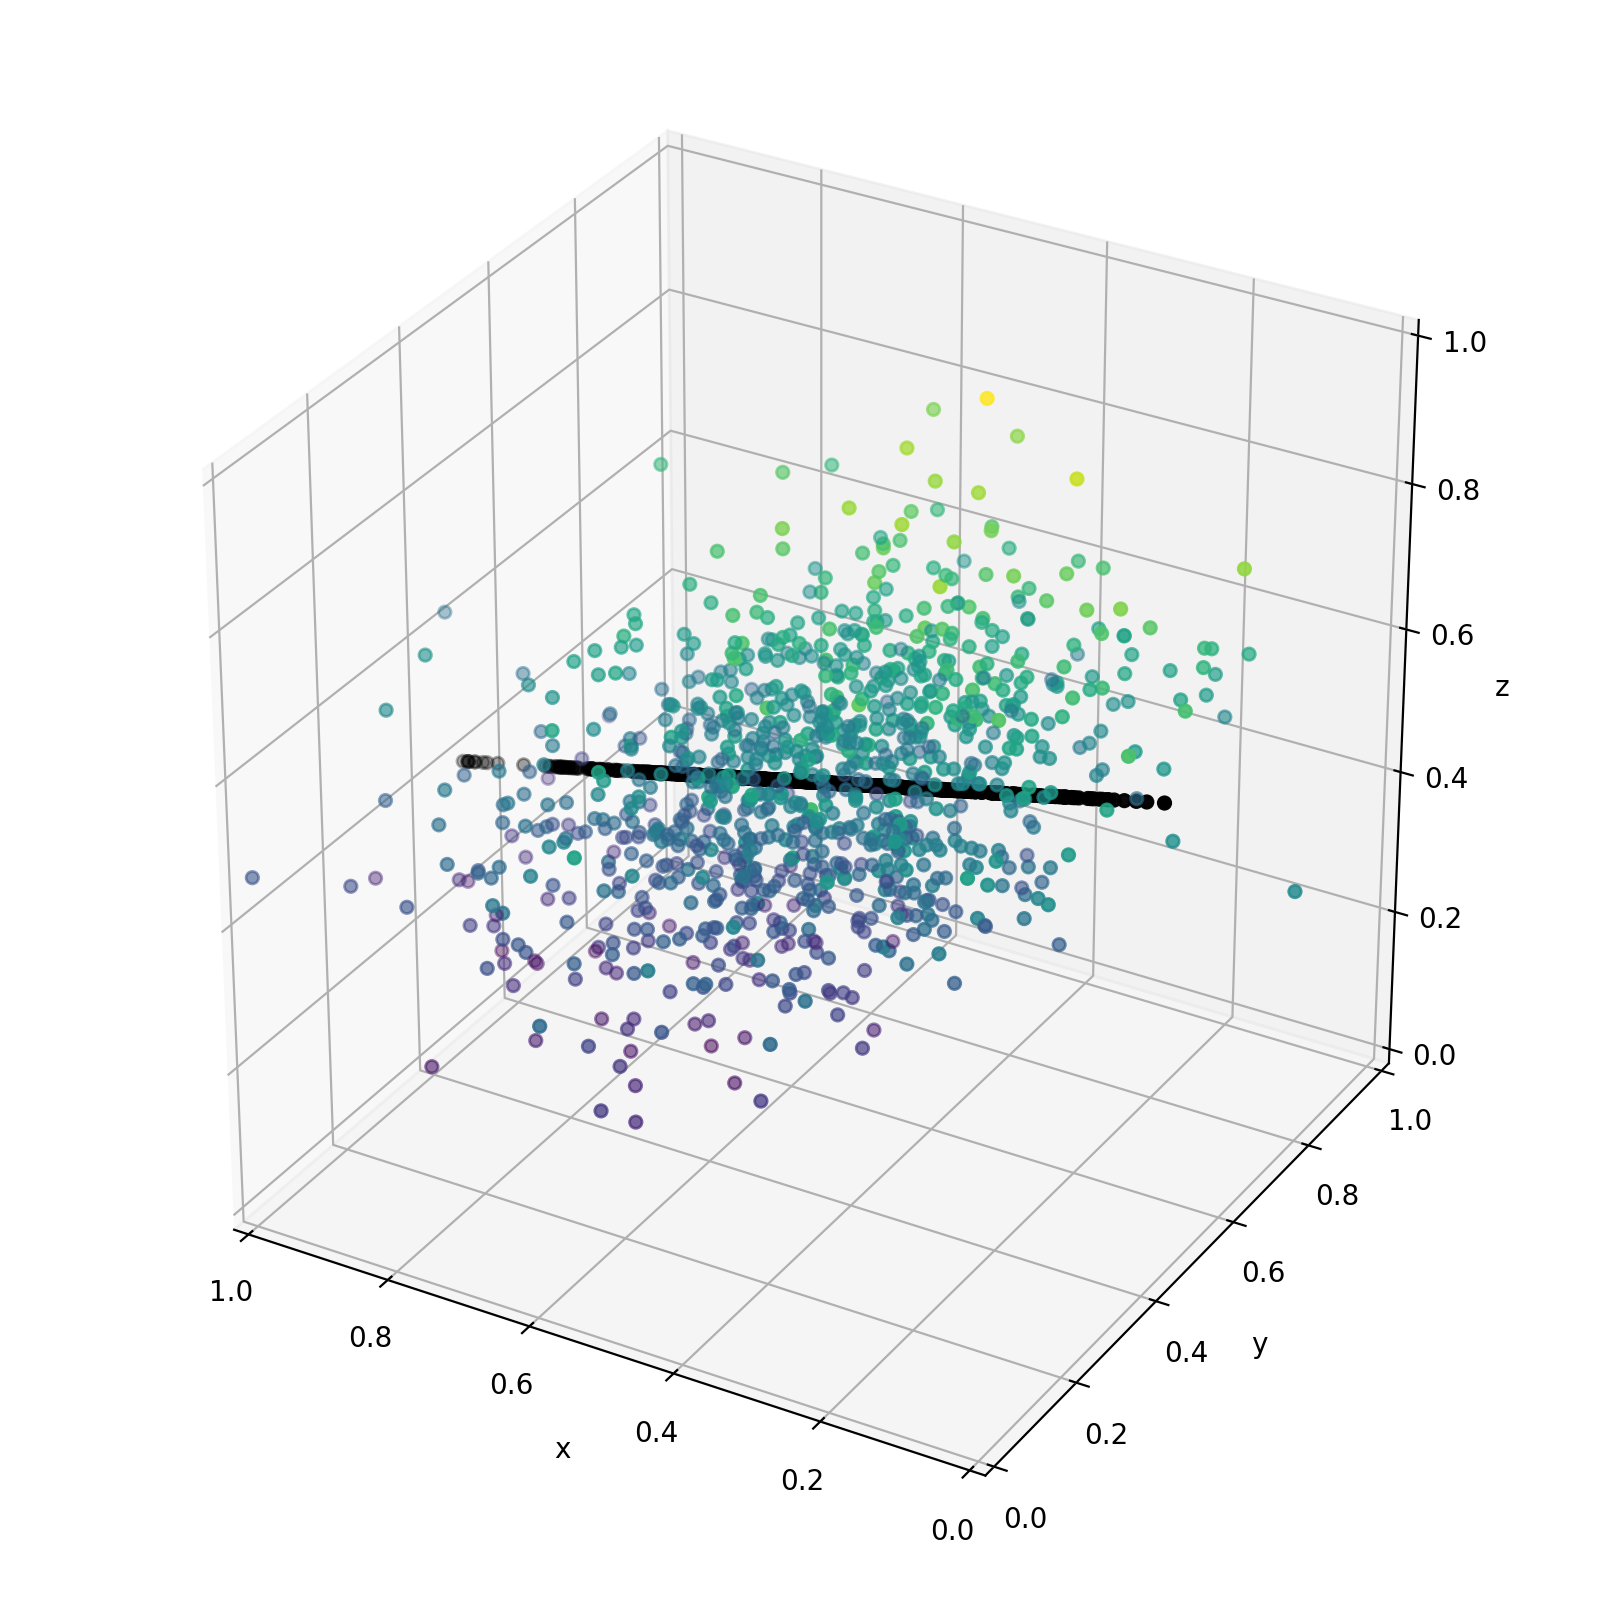
\includegraphics[width=\linewidth]{resources/X_Y_1_simulated.png}
		\caption{$\xx, \yy; \; t=1$}
		\label{fig:1}
	\end{subfigure}\hfil
	\begin{subfigure}{0.3\textwidth}
		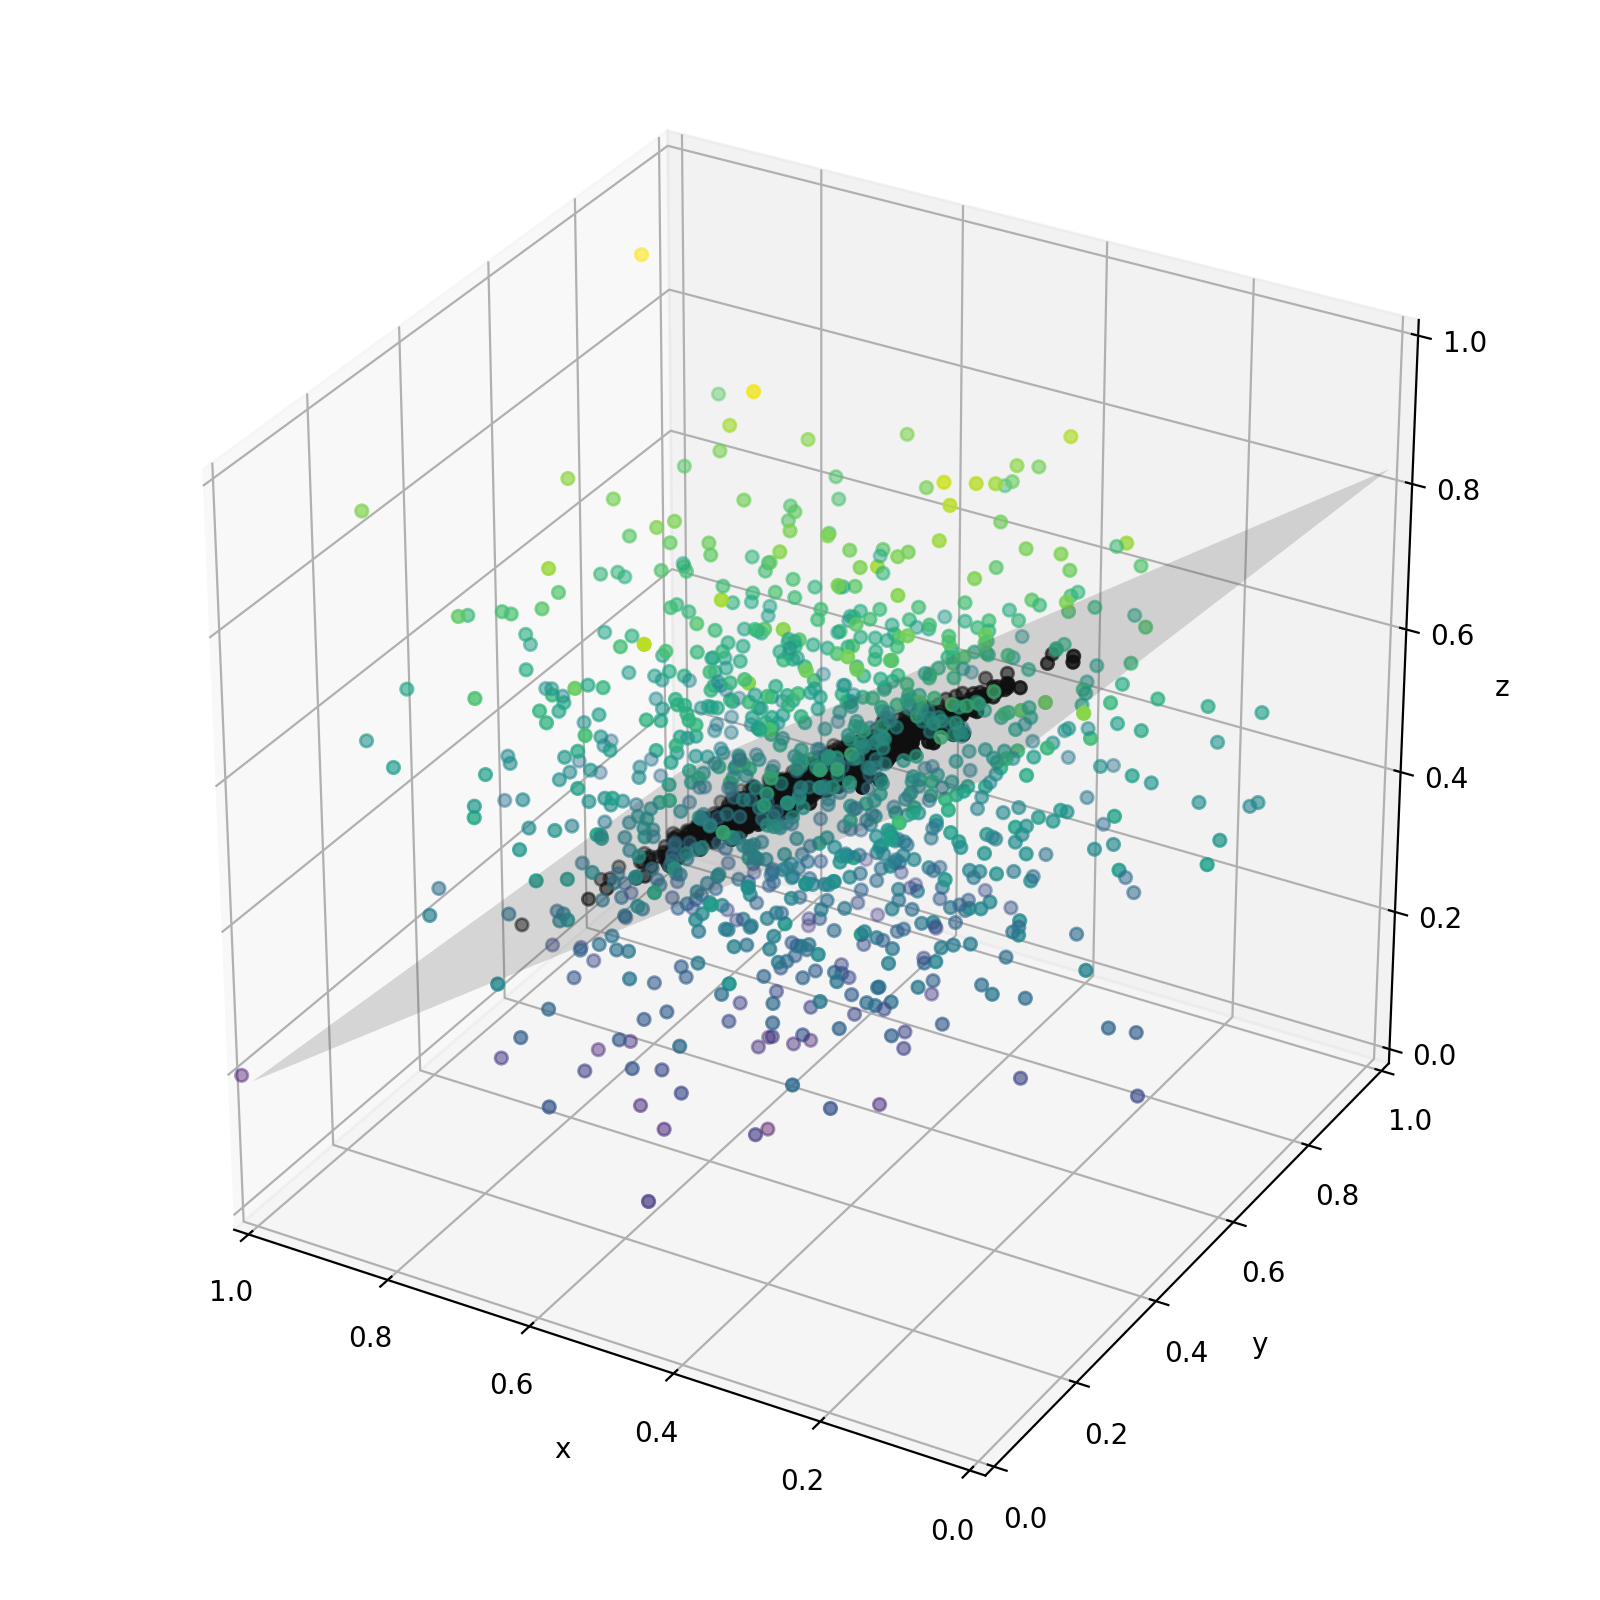
\includegraphics[width=\linewidth]{resources/X_Y_2_simulated.png}
		\caption{$\xx, \yy; \; t=2$}
		\label{fig:2}
	\end{subfigure}\hfil
	\begin{subfigure}{0.3\textwidth}
		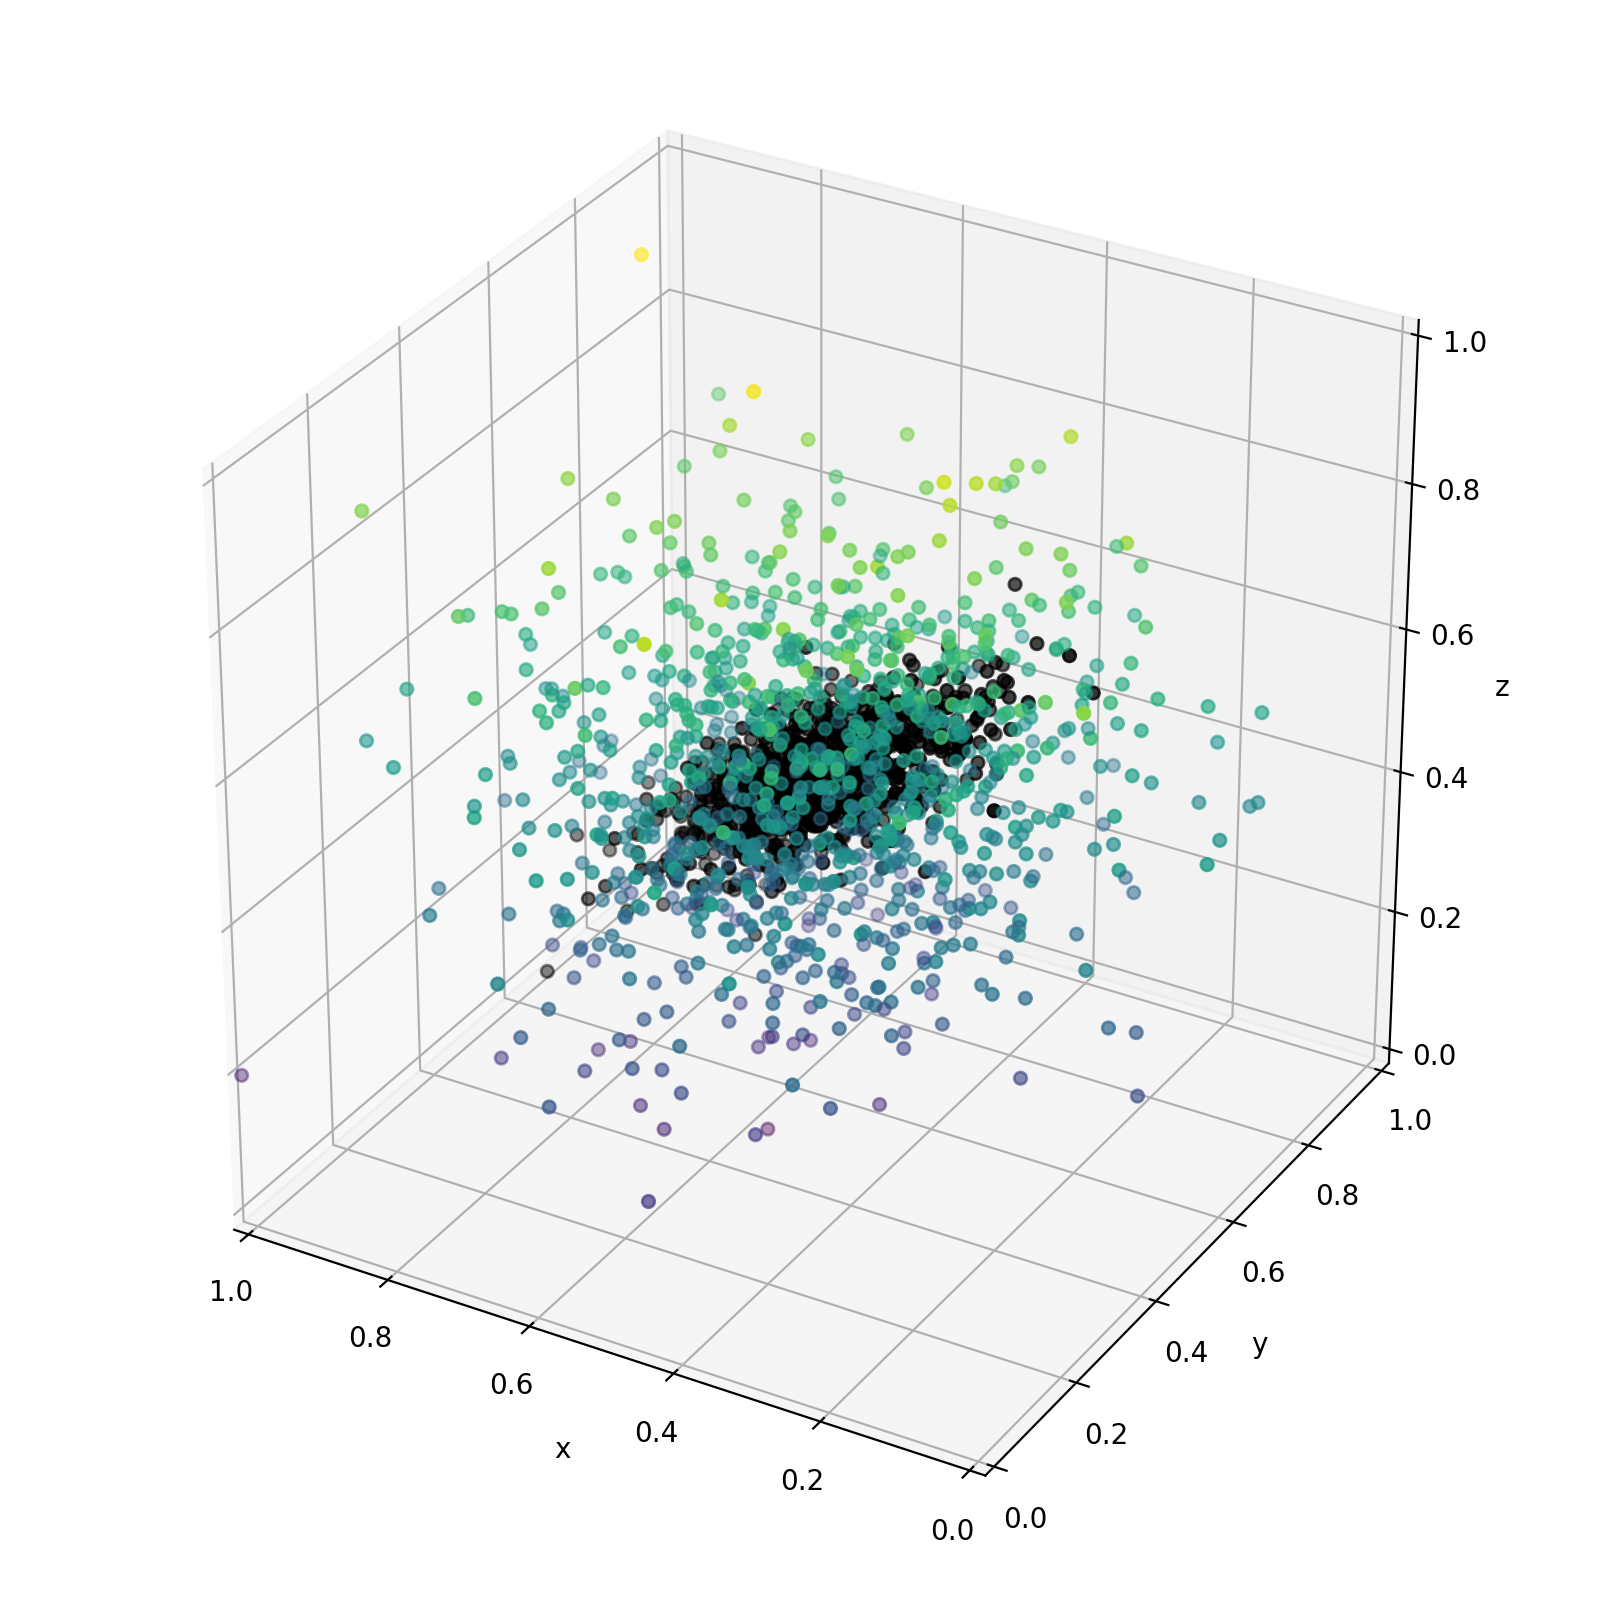
\includegraphics[width=\linewidth]{resources/X_Y_3_simulated.png}
		\caption{$\xx, \yy; \; t=3$}
		\label{fig:3}
	\end{subfigure}
	
	\medskip
	\begin{subfigure}{0.3\textwidth}
		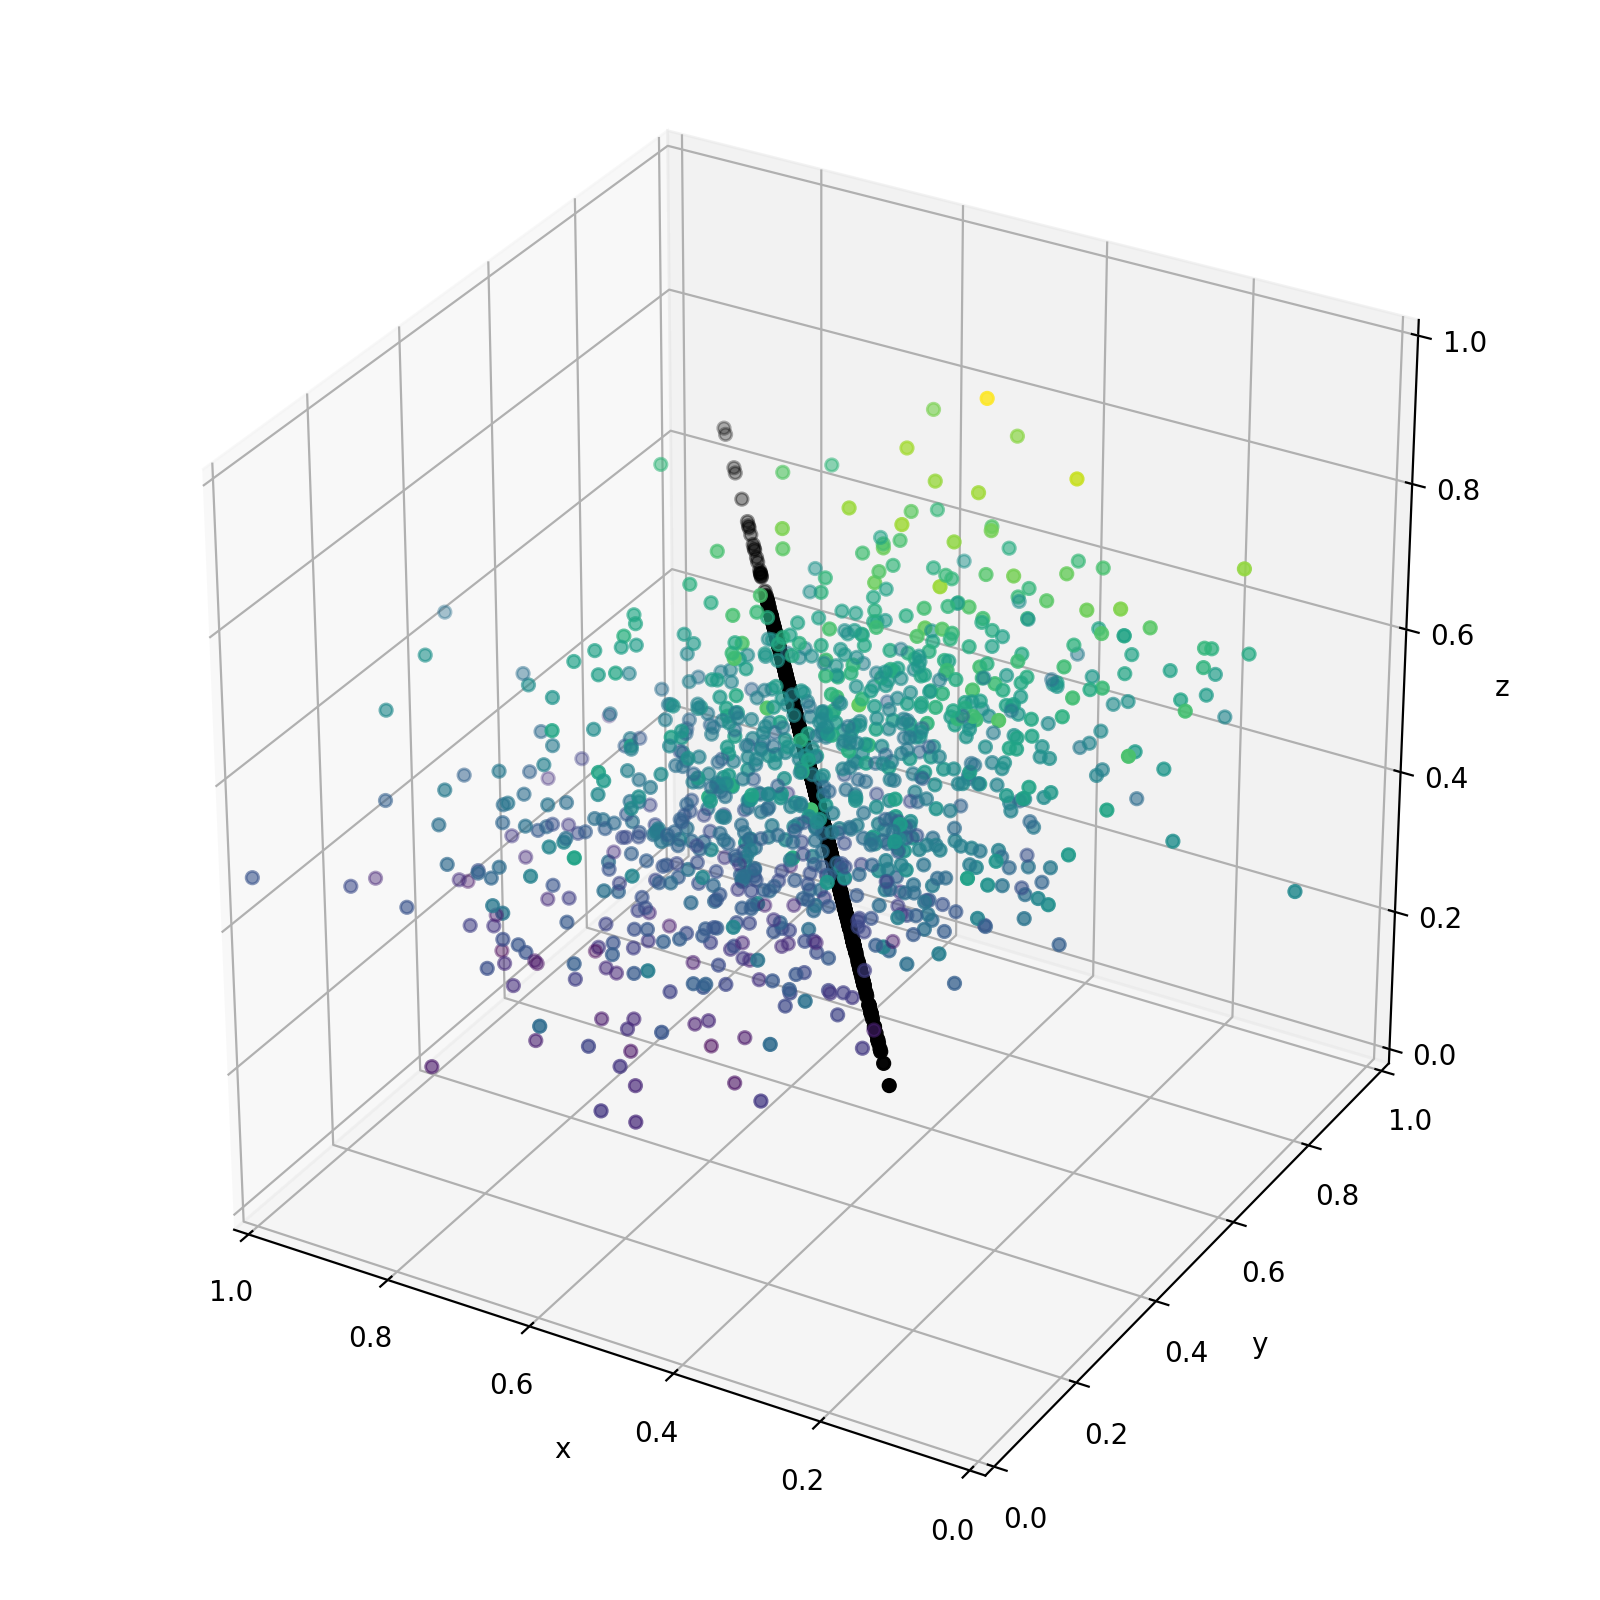
\includegraphics[width=\linewidth]{resources/Y_Y_1_simulated.png}
		\caption{$\yy, \yy; \; t=1$}
		\label{fig:4}
	\end{subfigure}\hfil
	\begin{subfigure}{0.3\textwidth}
		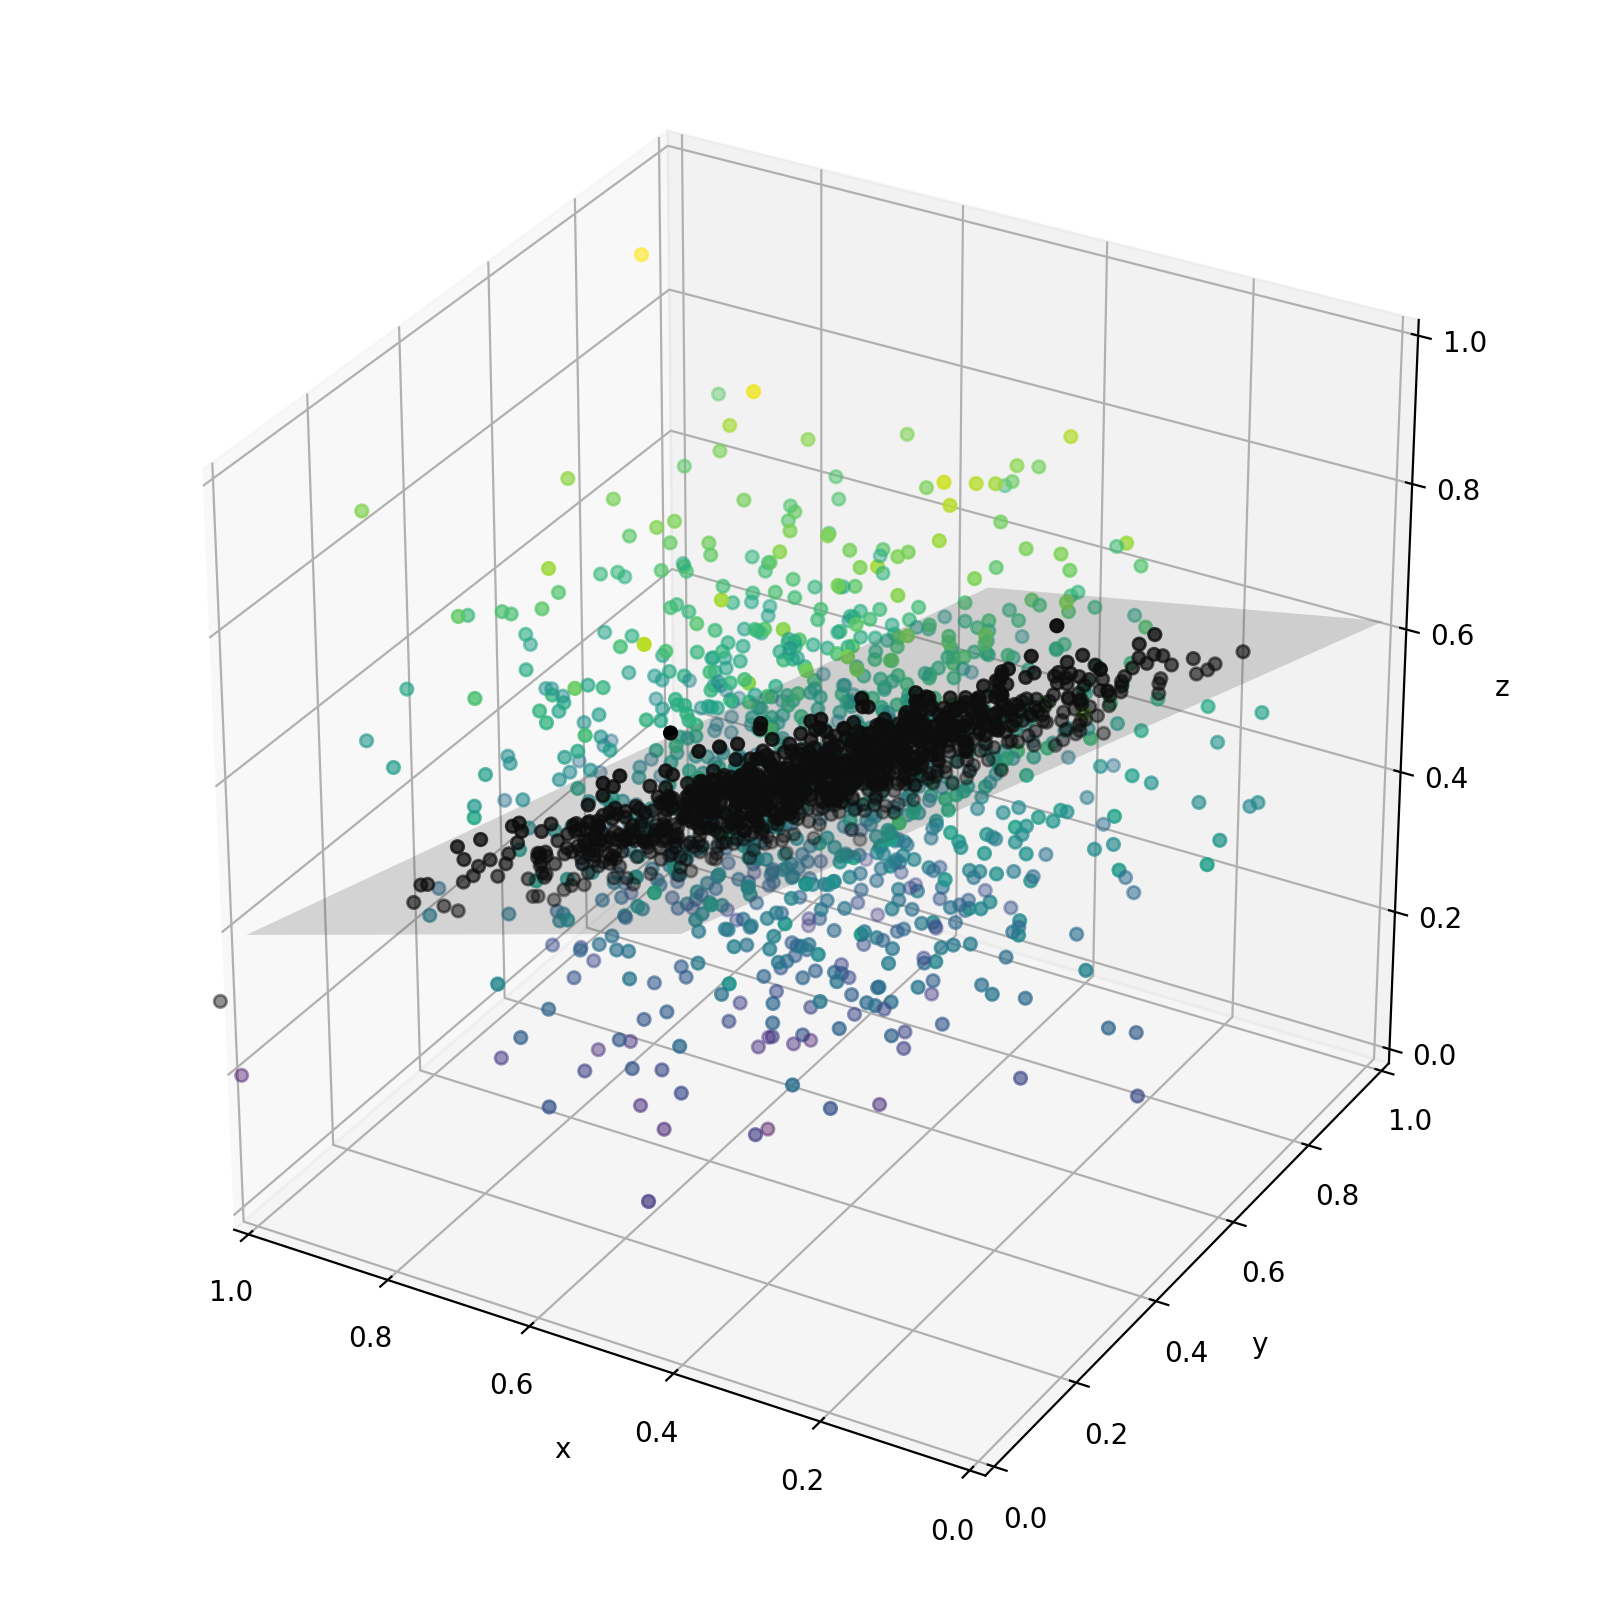
\includegraphics[width=\linewidth]{resources/Y_Y_2_simulated.png}
		\caption{$\yy, \yy; \; t=2$}
		\label{fig:5}
	\end{subfigure}\hfil
	\begin{subfigure}{0.3\textwidth}
		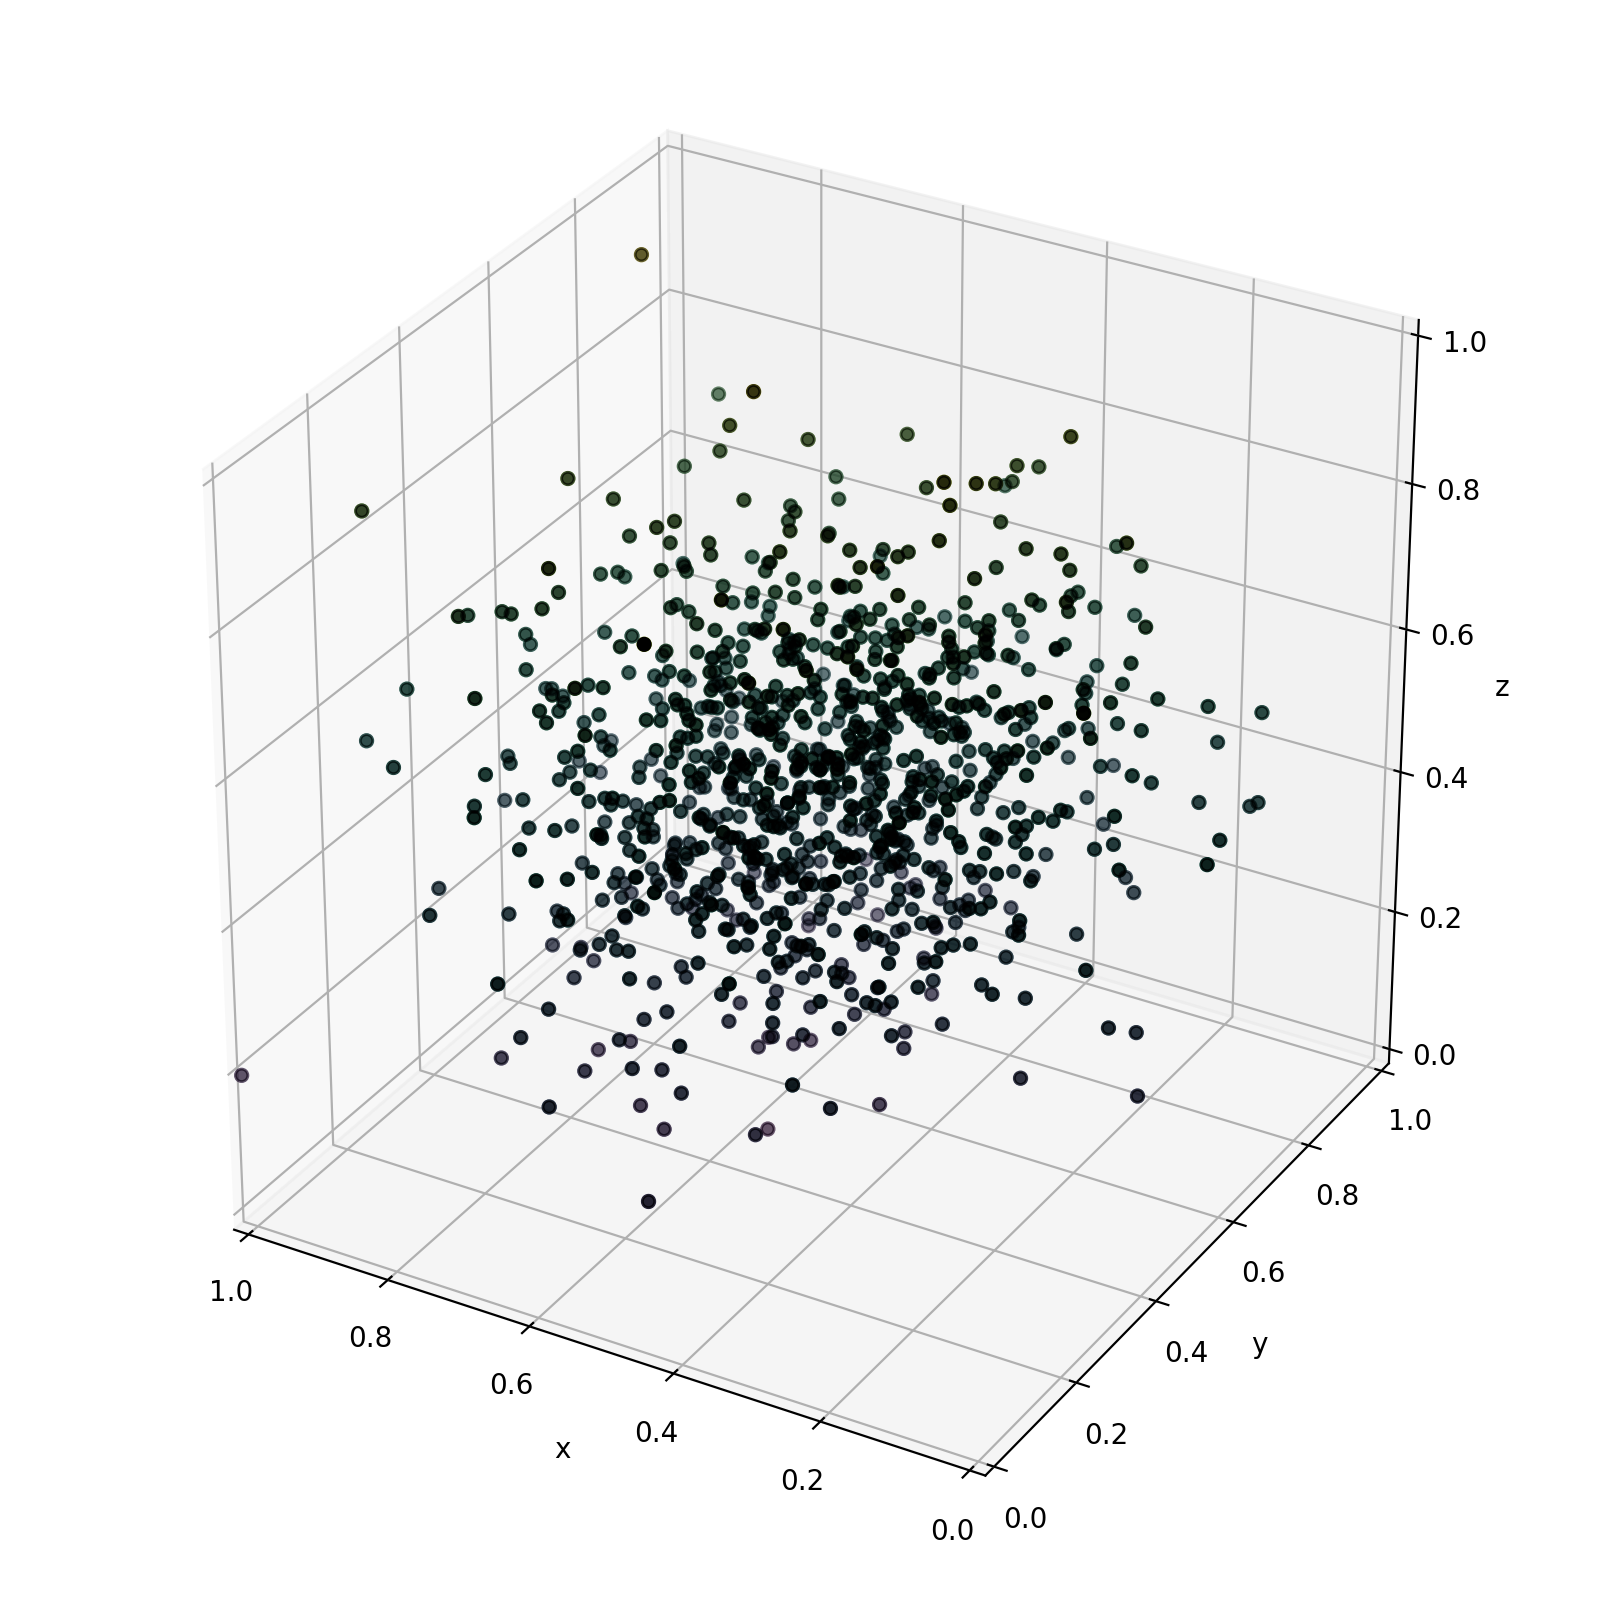
\includegraphics[width=\linewidth]{resources/Y_Y_3_simulated.png}
		\caption{$\yy, \yy; \; t=3$}
		\label{fig:6}
	\end{subfigure}
	\caption{Plots der Simulationen}
	\label{fig:images}
\end{figure}


\subsection*{Effektive Dimension der Regression}
Letztlich bleibt noch die Frage zu beantworten, wie man die sogenannte \textit{effektive Dimension} $t$ bei der Reduced-Rank-Regression geeignet wählen kann. Dafür beachte man, dass man in der Situation von Satz~\ref{thm:rrr}, wenn der Rang der Koeffizientenmatrix $t = t_0$ zu $t = t_1$, $\; t_0 < t_1$ vergrößert wird, eine Verringerung von $W_{t, \Ggamma}(\muu^{(t)}_{\min}, \A^{(t)}_{\min}, \B^{(t)}_{\min})$ der Höhe
$$W_{t_0, \Ggamma}(\muu^{(t_0)}_{\min}, \A^{(t_0)}_{\min}, \B^{(t_0)}_{\min}) - W_{t_1, \Ggamma}(\muu^{(t_1)}_{\min}, \A^{(t_1)}_{\min}, \B^{(t_1)}_{\min}) = \sum_{i=t_0+1}^{t_1} \lambda_i$$
bewirkt. Hiermit könnte man in der Praxis (wo man dann natürlich mit $\widehat{\lambda}_i$ arbeitet) untersuchen, bis wann es sich \glqq lohnt\grqq , 
$t$ zu vergrößern, was sich, wie in \cite[Seite 185]{Iz08} beschrieben wird, mit Tests, ob $\rk \, \Ggamma^{1/2} \Ssigma_{\Y\X} \Ssigma_{\X\X}^{-1} \Ssigma_{\X\Y} \Ggamma^{1/2} = \rk \, \Ssigma_{\Y\X}$ kleiner als eine festgelegte Zahl ist, überprüfen ließe. Ferner wird in \cite[Kapitel 6.3.4]{Iz08} ein anderer Algorithmus vorgestellt, mit dem die effektive Dimension $t$ bestimmt werden kann.



\newpage

\begin{thebibliography}{9}
	\bibitem[Iz08]{Iz08} 
	Izenman, Alan Julian.
	\textit{Modern Multivariate Statistical Techniques: Regression, Classification, and Manifold Learning}. 
	Springer Texts in Statistics, Springer-Verlag New York, 2008.
	\bibitem[BZ21]{BZ21}
	Bandeira, Afonso S. und Zhivotovskiy, Nikita.
	\textit{Lecture Notes for Mathematics of Machine Learning}. 2021.
	\url{https://metaphor.ethz.ch/x/2021/fs/401-2684-00L/sc/Math_of_ML_Lecture_Notes.pdf}
	\bibitem[EP73]{EP73}
	Eaton, Morris L. und Perlman, Michael D.
	\textit{The Non-Singularity of Generalized Sample Covariance Matrices}.
	The Annals of Statistics, 1973.
\end{thebibliography}



\end{document}
